% transposicoes
Um evento de transposição ocorre quando dois blocos adjacentes no
genoma trocam de posição. Uma transposição $\rho(i, j, k)$, para
$1 \leq i < j < k \leq n + 1$, aplicada ao genoma $\pi =
(~\pi_{1}~\pi_{2}~\ldots~\pi_{n}~)$ gera a permutação $\rho\pi =
(\pi_{1}~\ldots~\pi_{i-1}~\pi_{j}~\ldots~\pi_{k-1}~\pi_{i}~\ldots$
$\pi_{j-1}~\pi_{k}~\ldots~\pi_{n})$ (Figura~\ref{fig:transposition}).

\begin{figure}[h]
  \centering
  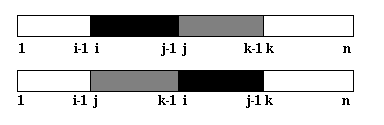
\includegraphics{images/transposition.png} 
  \caption{Transposição aplicada em uma permutação.}
  \label{fig:transposition}
\end{figure}

A distância de transposição $d_{t}(\pi, \sigma)$ entre duas
permutações $\pi$ e $\sigma$ é o número mínimo $t$ de transposições
$\rho_{1}, \rho_{2}, \ldots, \rho_{t}$ tal que
$\pi \rho_{1} \rho_{2} \ldots \rho_{t} = \sigma$. Note que a distância
de transposição entre $\pi$ e $\sigma$ é igual à distância de transposição
entre $\sigma^{-1} \pi$ e $\iota$. Então, sem perda de generalidade,
podemos dizer que o problema da distância de transposição é
equivalente ao problema de ordenação por transposições, que é a
distância de transposição entre a permutação $\pi$ e a permutação
identidade $\iota$, denotado por $d_{t}(\pi)$.

Este problema foi estudado por Bafna e
Pevzner~\cite{BafnaPevzner*1998}, onde apresentaram um algoritmo capaz
de fornecer uma resposta aproximada na razão de $1.5$, além de derivar
um importante limitante inferior para o problema. Introduziram o
conceito de \bkp{} em eventos de transposições, elementos adjacentes
em um genoma, mas não no outro, e o conceito de grafo de ciclos, ambos
ferramentas importantes utilizadas para encontrar limitantes para o
problema. Foram apresentados várias questões em aberto como verificar
a complexidade do problema da distância de transposição e o diâmetro,
que é a maior distância possível entre duas permutações de tamanho
$n$. O problema do diâmetro foi estudado por Meidanis, Walter e
Dias~\cite{MeidanisWalterDias*1997}.

A complexidade deste problema ficou em aberto por um longo tempo. O
trabalho de Bulteau, Fertin e Rusu~\cite{BulteauFertinRusu*2010}
apresentou a prova de que o problema de ordenação por transposição
pertence a classe dos problemas NP-Difíceis. Elias e
Hartman~\cite{EliasHartman*2006} apresentaram um algoritmo de
aproximação na razão de $1.375$. O trabalho de
Labarre~\cite{Labarre*2006} apresentou novos limitantes, além de
definir classes de permutações em que a distância de transposição pode
ser calculada em tempo e espaço lineares.

Nas subseções~\ref{subsec:trans_bkp} e~\ref{subsec:trans_cycle_graph}
apresentam ferramentas usadas para encontrar limitantes para o
problema de ordenação por transposições. Os limitantes usados neste
projeto estão descritos na subseção~\ref{subsec:trans_limitantes}.

\subsection{Breakpoints}
\label{subsec:trans_bkp}
No problema de ordenação por transposições, um \bkp{} é um par
$(\pi_{i}, \pi_{i+1})$ tal que $\pi_{i+1} \neq \pi_{i} + 1$. Denota-se
por $b_{t}(\pi)$ como sendo o número de \bkp{} na permutação $\pi$.

\subsection{Grafo de ciclos}
\label{subsec:trans_cycle_graph}
O conceito de grafo de ciclos foi introduzido por Bafna e
Pevzner~\cite{BafnaPevzner*1998} e foi usado para obter limitantes
melhores para o problema.

Um grafo direcionado com arestas coloridas, denotado por $G(\pi)$, é
chamado de grafo de ciclos da permutação $\pi$ se possui um conjunto
de vértices $\{0,~1,~\ldots~,~n+1\}$ e seu conjunto de arestas é
definido como para todo $1 \leq i \leq n+1$, arestas cinzas são
direcionadas de $i-1$ para $i$ e arestas pretas de $\pi_{i}$ para
$\pi_{i-1}$. A Figura~\ref{fig:trans_cycle_graph} mostra o grafo de
ciclos para a permutação $\pi = (~4~7~3~6~2~5~1~)$.

\begin{figure}[h]
  \centering 
  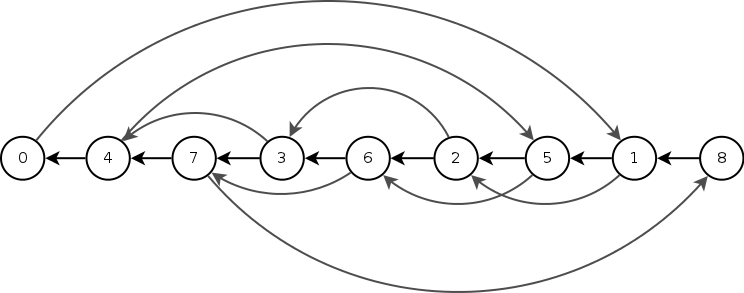
\includegraphics[scale=0.6]{images/trans_cycle_graph.png} 
  \caption{Grafo de ciclos para a permutação $\pi = (~4~7~3~6~2~5~1~)$.}
  \label{fig:trans_cycle_graph}
\end{figure}

\subsection{Limitantes}
\label{subsec:trans_limitantes}
Para o problema de ordenação por transposições usamos três tipos de
limitantes:

\begin{itemize}
\item{\textit{tra\_def}. 
Este é o limitante padrão, com limite inferior igual à $0$ e limite
superior igual a $n$ (tamanho da permutação).}
\item{\textit{tra\_br}.
Usando o conceito de \bkp{} em transposições, sabemos que uma
transposição atua em três pontos de uma permutação, logo, pode reduzir
o número de \bkp{} em pelo menos um e no máximo
três~\cite{BafnaPevzner*1998}, levando ao
Teorema~\ref{teo:trans_br_bound}.

\begin{teo}
  \label{teo:trans_br_bound}
  Para qualquer permutação $\pi$, $\frac{b_t(\pi)}{3} \leq d_t(\pi) \leq
  b_t(\pi)$.
\end{teo}
}
\item{\textit{tra\_cg}.
Usando o conceito de grafo de ciclos, um ciclo alternado de $G(\pi)$ é
ciclo direcionado com arestas de cores alternadas. Para todo vértice
de $G(\pi)$ toda aresta chegando é unicamente pareada com uma aresta
saindo de cor diferente. Isto implica que existe uma decomposição
única de ciclos alternados do conjunto de arestas de $G(\pi)$. A
seguir o termo ciclo é usado no lugar de ciclos alternados e usamos o
termo $k-\text{ciclo}$ para definir um ciclo alternado de tamanho $2k$,
$k-\text{ciclo}$ é longo se $k > 2$, e curto caso contrário.

Para melhorar o limitante, Bafna e Pevzner~\cite{BafnaPevzner*1998}
estudou separadamente os ciclos pares e ímpares. Um ciclo é impar se
número ímpar de arestas pretas e par caso contrário. Seja
$c_{ímpar}(\pi)$ o número de ciclos ímpares de $G(\pi)$, para uma
permutação $\pi$, e $\Delta c_{ímpar} (\rho) = c_{ímpar} (\pi \rho) -
c_{ímpar} (\pi)$ a mudança no número de ciclos ímpares devido a
transposição $\rho$, temos que $\Delta c_{ímpar} \in \{2, 0, -2\}$,
gerando o resultado do Teorema~\ref{teo:trans_cg_bound}.

\begin{teo} 
  \label{teo:trans_cg_bound} 
  Para qualquer permutação $\pi$, $\frac{n + 1 - c_{ímpar}(\pi)}{2} \leq
  d_t(\pi) \leq \frac{3}{4} (n + 1 - c_{ímpar}(\pi))$.
\end{teo}
}
\end{itemize}
